
%(BEGIN_QUESTION)
% Copyright 2015, Tony R. Kuphaldt, released under the Creative Commons Attribution License (v 1.0)
% This means you may do almost anything with this work of mine, so long as you give me proper credit

\noindent

\vskip 5pt


\textbf{Introduksjon}

I dette arbeidsoppdraget skal du jobbe med målesystemer for nivå. Du skal utføre sjekk og kalibrering for nivåmålesystemer basert på følgende prinsipper:
\begin{itemize}[noitemsep]
	\item Ultralyd
	\item Trykk
	\item Radar
\end{itemize}

%$$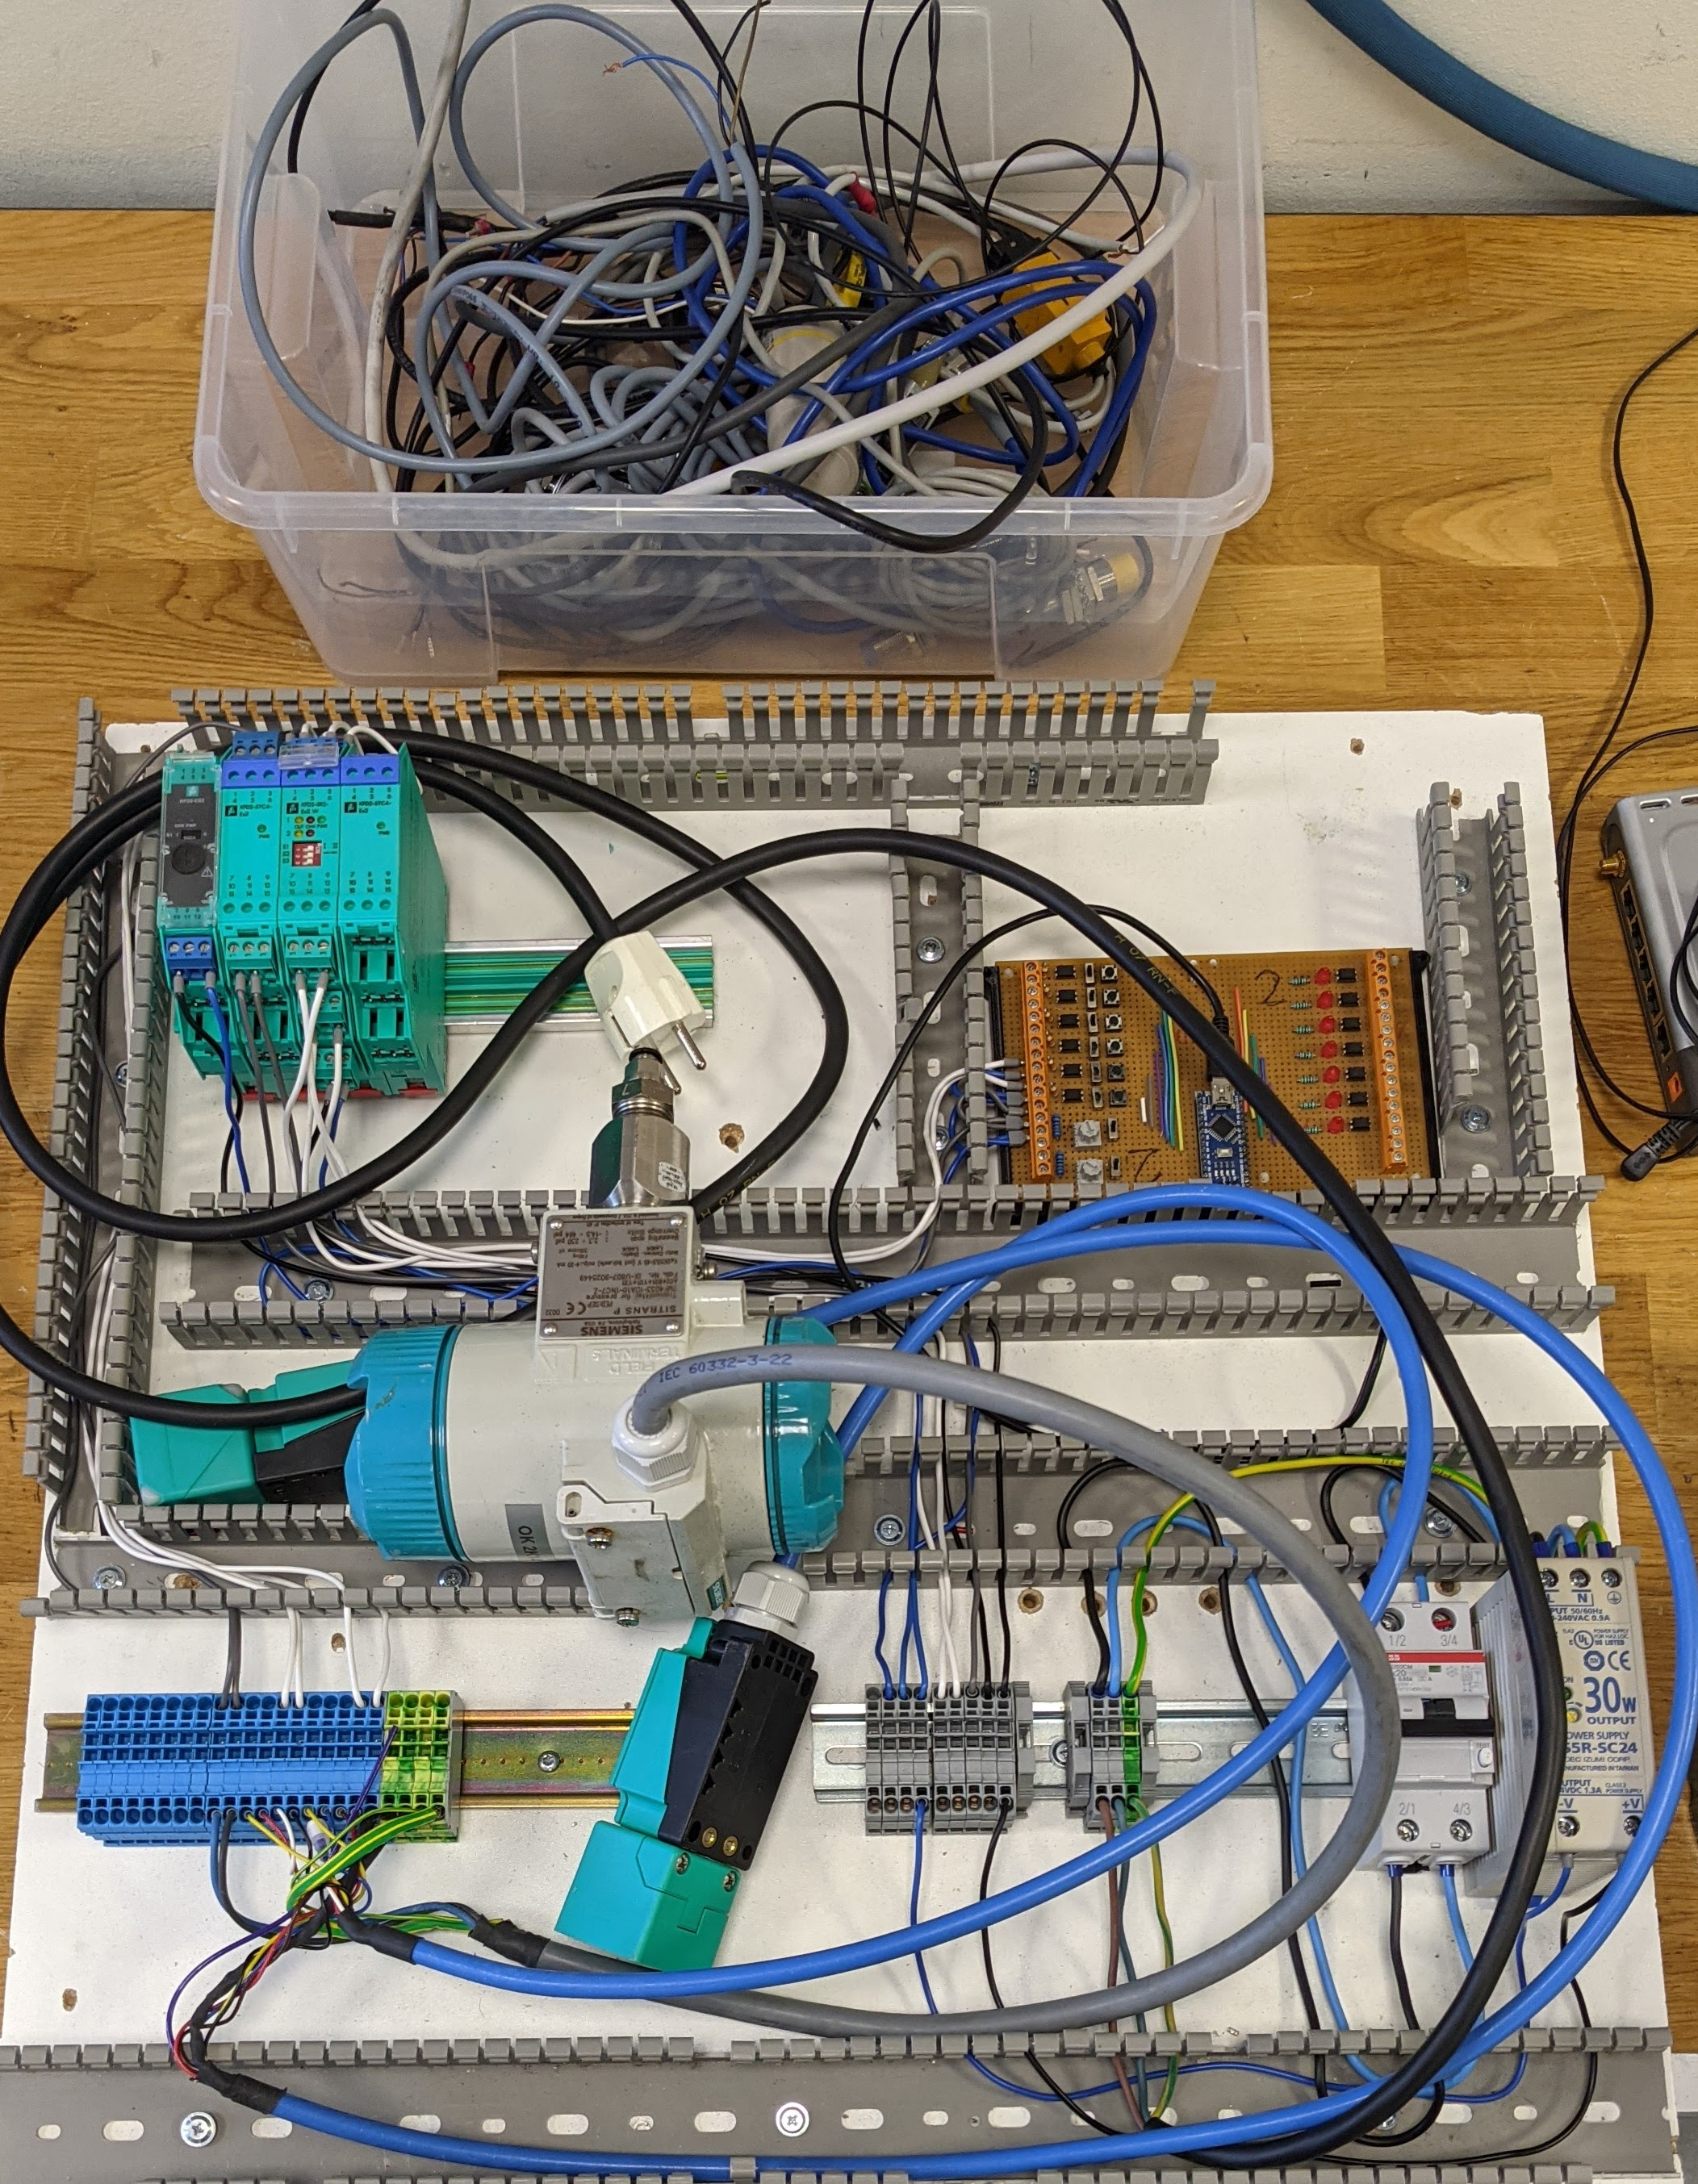
\includegraphics[width=13cm]{i04823x01.jpg}$$\\
\textbf{Kalibrering og justering range for en smart transmitter}
Målet med oppgaven er å lære hvordan vi justerer en transmitter for trykk.



\textbf{Teorioppgaver}
\href {https://autofaget.no/level/node2.html} {Leseoppgave}
\textbf{Planlegging}


\textbf{Gjennomføring}

\textbf{Dokumentasjon}

\begin{enumerate}
	\item Beskriv hvordan du planla, gjennomførte og dokumentere jobben. Forklar eventuelle avvik dere måtte observere under oppdraget. 
\end{enumerate}










\vfil 


\underbar{file i04843}
\vfil \eject
%(END_QUESTION)





%(BEGIN_ANSWER)


%(END_ANSWER)





%(BEGIN_NOTES)


%INDEX% Arbeisdoppdrag, Målesystemer, Nivå 1, Stasjon10, Kalibrering, DP-celle(Smart)

%(END_NOTES)


